%% Template for ENG 401 reports
%% by Robin Turner
%% Adapted from the IEEE peer review template

%
% note that the "draftcls" or "draftclsnofoot", not "draft", option
% should be used if it is desired that the figures are to be displayed in
% draft mode.

\documentclass[peerreview]{IEEEtran}
\usepackage{cite} % Tidies up citation numbers.
\usepackage{url} % Provides better formatting of URLs.
\usepackage{booktabs} % Allows the use of \toprule, \midrule and \bottomrule in tables for horizontal lines
\usepackage{graphicx}
\usepackage{amsmath}
\usepackage{amsfonts}
\usepackage{amssymb}

\usepackage[T1]{fontenc}
%\usepackage[Polish]{babel}
\usepackage[utf8]{inputenc}

\usepackage{lipsum}

\graphicspath{.}


\hyphenation{op-tical net-works semi-conduc-tor} % Corrects some bad hyphenation 



\begin{document}
%\begin{titlepage}
% paper title
% can use linebreaks \\ within to get better formatting as desired
\title{Raport z badania CFD\\ trzech wariantów geometrycznych przekładek}


% author names and affiliations

\author{Lewandowska Natalia \\
Katedra Techniki Cieplnej\\
Politechnika Poznańska\\
}
\date{\today}

% make the title area
\maketitle
\tableofcontents
\listoffigures
\listoftables
%\end{titlepage}

\IEEEpeerreviewmaketitle

\begin{abstract}

\lipsum[1]

\end{abstract}





\section{Wstęp}
This will be a revised version of the introduction in your proposal.

\section{Opis problemu badawczego}
This will be a revised version of the problem definition in your proposal.


\begin{figure}[!h]
\centering
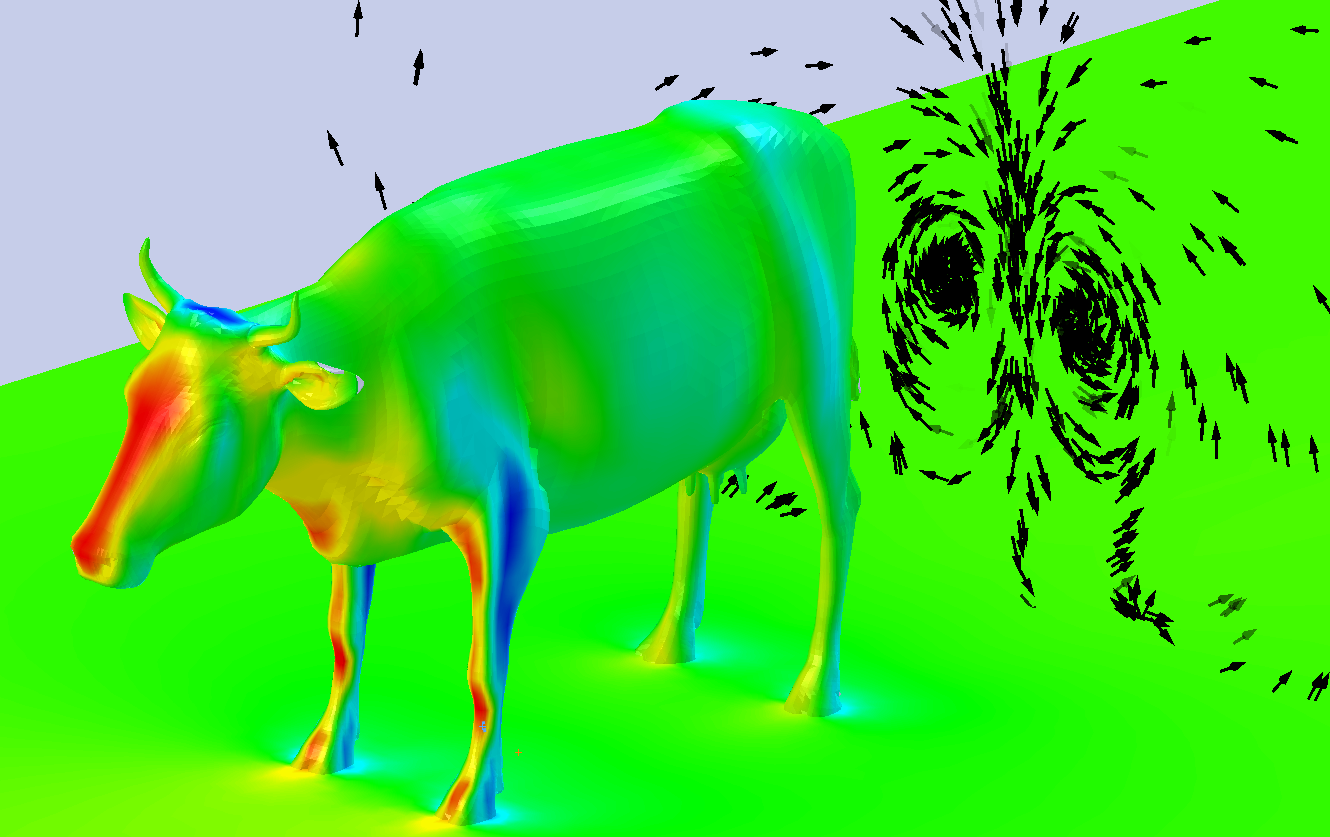
\includegraphics[width=0.8\columnwidth]{placeholder} 
\caption{Simulation Results}
\label{fig_sim}
\end{figure}

% Note that IEEE typically puts floats only at the top, even when this
% results in a large percentage of a column being occupied by floats.

\section{Metodyka badań - pre-processing, processing}
This may be a modified version of your proposal depending on previously carried out research or any feedback received.  
\subsection{Warunki brzegowe, geometria}
Describe your first solution here.
\subsection{Siatka obliczeniowa}
Describe your second solution here.
\subsection{Model analityczny, model turbulencji}
\subsection{Parametry solvera numerycznego??}

opisuje się solver w takich przypadkach? może grafiki resiudów?



\section{Wyniki badań CFD} \label{sec:criteria}
\subsection{Rozkłady prędkości na wlocie, w połowie długości przekładki i na wylocie}
tutaj obrazki przekrojów z CFD, wykresy rozkładu, 

wartości area weighted average prędkości??

\subsection{Rozkłady prędkości i ciśnienia wzdłuż przekładek}

oprócz obrazków tutaj by trzeba oszacować jakiś parametr mówiący miejscach stangnacji --> proponuję obliczyć procent objętości przestrzeni w zakładce, w której prędkość jest równa zero, inne propozycje? wyniki zestawić w tabeli



\section{Walidacja obliczeń numerycznych}
tu w sumie nie wiem co napsać, bo raport nie obejmował eksperymentu
%\begin{itemize}
%\item Relevance to the context of application  
%\end{itemize}
 


\section{Analiza i interpetacja wyników badań}

która najlepsza, która najgorsza 


wzór tabeli (zostawiam sobie, może się przyda):

% Example of a table from http://www.latextemplates.com/template/professional-table
\begin{table} % Add the following just after the closing bracket on this line to specify a position for the table on the page: [h], [t], [b] or [p] - these mean: here, top, bottom and on a separate page, respectively
\centering % Centers the table on the page, comment out to left-justify
\begin{tabular}{l c c c c c} % The final bracket specifies the number of columns in the table along with left and right borders which are specified using vertical bars (|); each column can be left, right or center-justified using l, r or c. To specify a precise width, use p{width}, e.g. p{5cm}
\toprule % Top horizontal line
& \multicolumn{5}{c}{Growth Media} \\ % Amalgamating several columns into one cell is done using the \multicolumn command as seen on this line
\cmidrule(l){2-6} % Horizontal line spanning less than the full width of the table - you can add (r) or (l) just before the opening curly bracket to shorten the rule on the left or right side
Strain & 1 & 2 & 3 & 4 & 5\\ % Column names row
\midrule % In-table horizontal line
GDS1002 & 0.962 & 0.821 & 0.356 & 0.682 & 0.801\\ % Content row 1
NWN652 & 0.981 & 0.891 & 0.527 & 0.574 & 0.984\\ % Content row 2
PPD234 & 0.915 & 0.936 & 0.491 & 0.276 & 0.965\\ % Content row 3
JSB126 & 0.828 & 0.827 & 0.528 & 0.518 & 0.926\\ % Content row 4
JSB724 & 0.916 & 0.933 & 0.482 & 0.644 & 0.937\\ % Content row 5
\midrule % In-table horizontal line
\midrule % In-table horizontal line
Average Rate & 0.920 & 0.882 & 0.477 & 0.539 & 0.923\\ % Summary/total row
\bottomrule % Bottom horizontal line
\end{tabular}
\smallskip 
\caption{Some impressive numbers} % Table caption, can be commented out if no caption is required
\label{tab:template} % A label for referencing this table elsewhere, references are used in text as \ref{label}
\end{table}
A reference to Table \ref{tab:template}.

\section{Propozycja poszerzenia badań}

czyli badania na całej komorze




%\appendices
%\section{What Goes in the Appendices} \label{App:WhatGoes}
%The appendix is for material that readers only need to know if they are studying the report in depth. Relevant charts, big tables of data, large maps, graphs, etc. that were part of the research, but would distract the flow of the report should be given in the Appendices. 
%\section{Formatting the Appendices} \label{App:Formatting}
%Each appendix needs to be given a letter (A, B, C, etc.) and a title. \LaTeX will do the lettering automatically.


\begin{thebibliography}{1}
% Here are a few examples of different citations 
% Book
\bibitem{kopka_1999} % Note the label in the curly brackets. Use the cite the source; e.g., \cite{kopka_latex}
H.~Kopka and P.~W. Daly, \emph{A Guide to \LaTeX}, 3rd~ed.\hskip 1em plus
  0.5em minus 0.4em\relax Harlow, England: Addison-Wesley, 1999.
\bibitem{horowitz_2005}D.~Horowitz, \emph{End of Time}. New York, NY, USA: Encounter Books, 2005. [E-book] Available: ebrary, \url{http://site.ebrary.com/lib/sait/Doc?id=10080005}. Accessed on: Oct. 8, 2008.
% Article from database
\bibitem{castlevecchi_2008}D.~Castelvecchi, ``Nanoparticles Conspire with Free Radicals'' \emph{Science News}, vol.174, no. 6, p. 9, September 13, 2008. [Full Text]. Available: Proquest, \url{http://proquest.umi.com/pqdweb?index=52&did=1557231641&SrchMode=1&sid=3&Fmt=3&VInst=PROD&VType=PQD&RQT=309&VName=PQD&TS=1229451226&clientId=533}. Accessed on: Aug.~3, 2014.
% Conference Paper from the Internet
\bibitem{lach_2010}J.~Lach, ``SBFS: Steganography based file system,'' in \emph{Proceedings of the 2008 1st International Conference on Information Technology, IT 2008, 19-21 May 2008, Gdansk, Poland.} Available: IEEE Xplore, \url{http://www.ieee.org}. [Accessed: 10 Sept. 2010].
% Web page, no author
\bibitem{a_laymans_explanation}``A `layman's' explanation of Ultra Narrow Band technology,'' Oct.~3, 2003. [Online]. Available: \url{http://www.vmsk.org/Layman.pdf}. [Accessed: Dec.~3, 2003]. 
\end{thebibliography}

% This is a hand-made bibliography. If you want to use a BibTeX file, you're on your own ;-)














\end{document}
